\section{Research Methods}
\label{chap:research_methods}
In this chapter, general research theory, including data generation, data analysis, and sampling, will be presented. The learnings will help us answer the research questions and goals defined in the previous chapter.

\subsection{Research Model}
\citeauthor{oates_researching_2006} presents an overview model of the research process in her “Researching information systems and computing” book. This model illustrates the flow of a research process, including defining the research, strategies, data generation methods, and data analysis. Figure \ref{fig:research_process} illustrates this model where the components we have used in our research are shaded blue.

\begin{figure}[H]
    \centering
    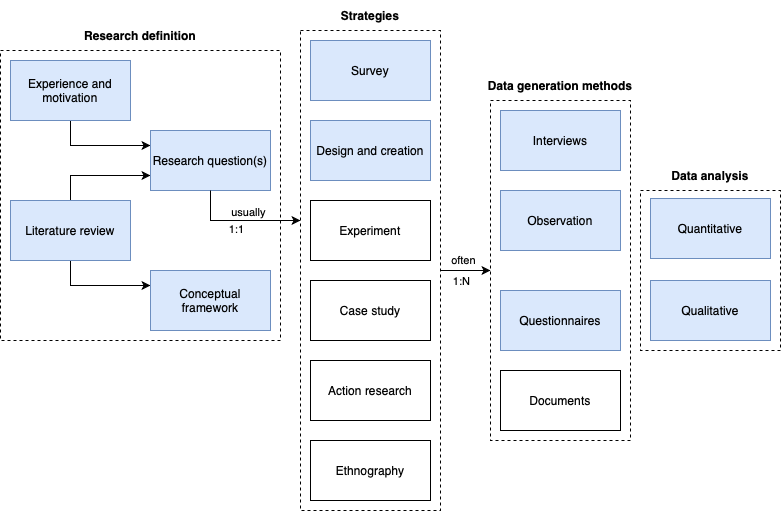
\includegraphics[width=0.8\textwidth]{Images/ResearchMethods/ResearchProcess.png}
    \caption{Model of the research process. Components we used are shaded blue \citep{oates_researching_2006}.}
    \label{fig:research_process}
\end{figure}

\subsection{Experience and Motivation}
\subsection{Literature Review}
\subsection{Research Questions}
\subsection{Conceptual Framework}
\subsection{Strategies}
\subsection{Data Generation Methods}
\subsection{Data Analysis}
\subsection{Summary}